\chapter{Metodolog'ia de desarrollo y calid'ad}
\section{An'alisis}
\subsection{Requerimientos funcionales}

\subsection{Requerimientos no funcionales}

\section{Dise'no}
\subsection{Casos de uso}

\subsection{Mockup}
\begin{center}
\begin{figure}
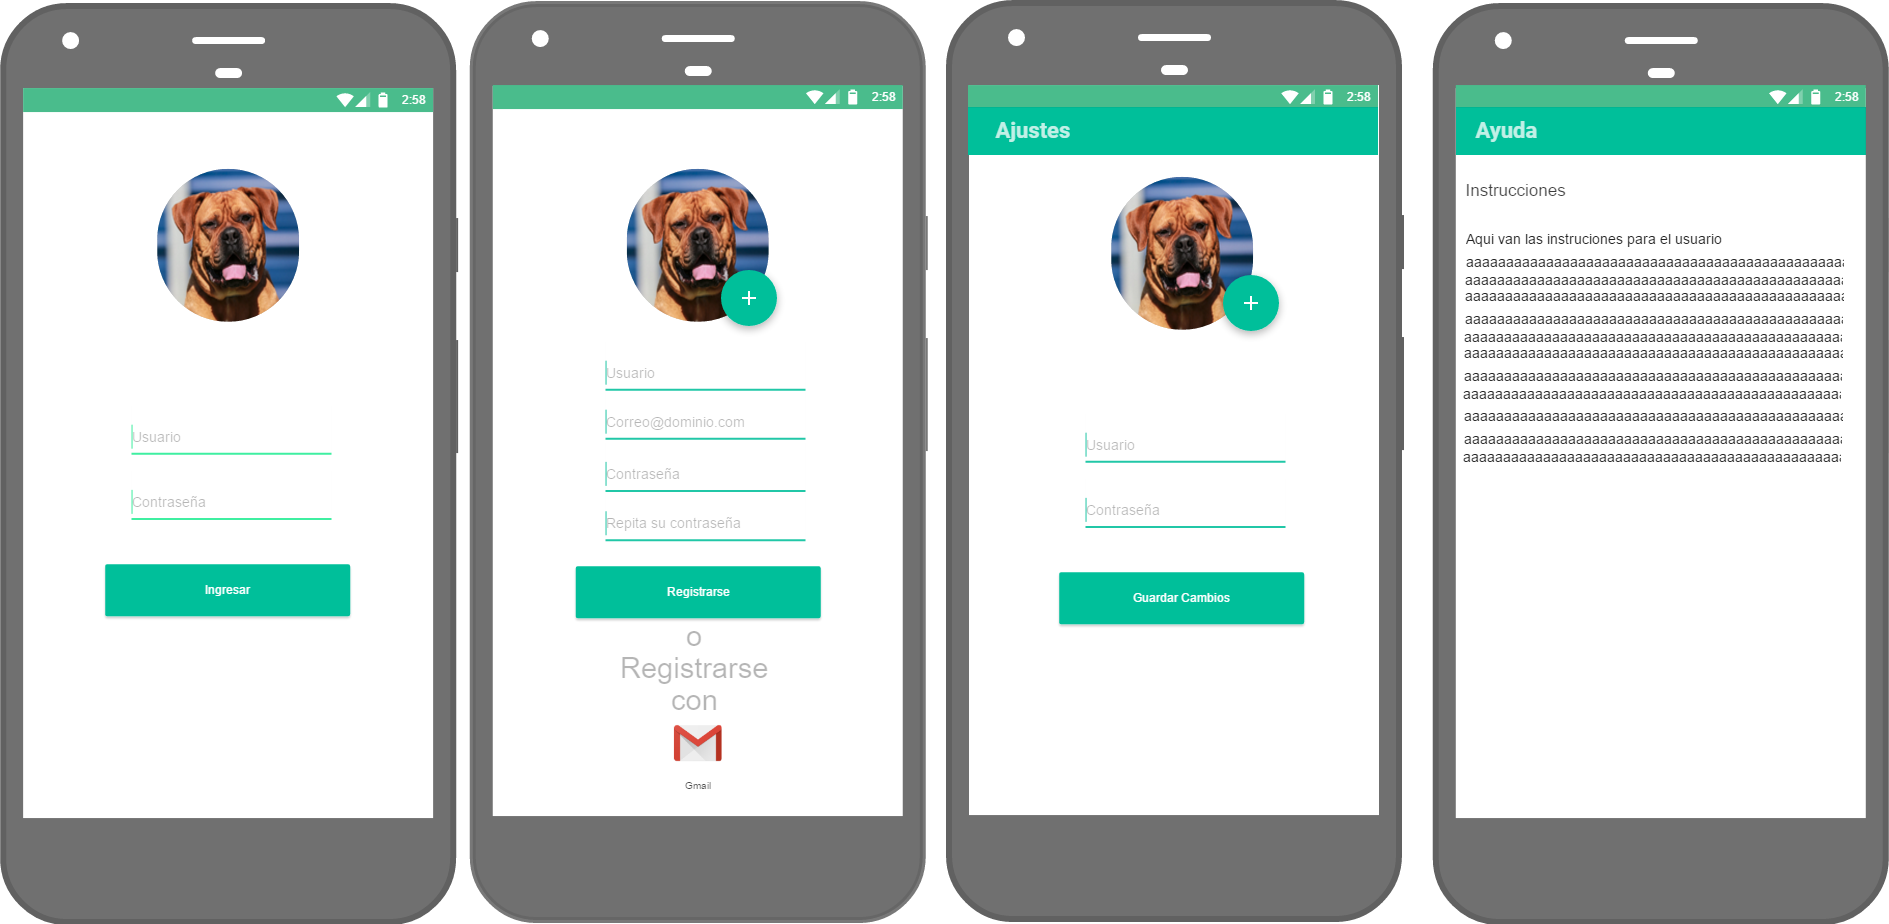
\includegraphics[scale=0.2]{img/m1.png} 
\caption{Pantallas de inicio de sesión y sección de ayuda}
\end{figure}
\end{center}

\begin{center}
\begin{figure}
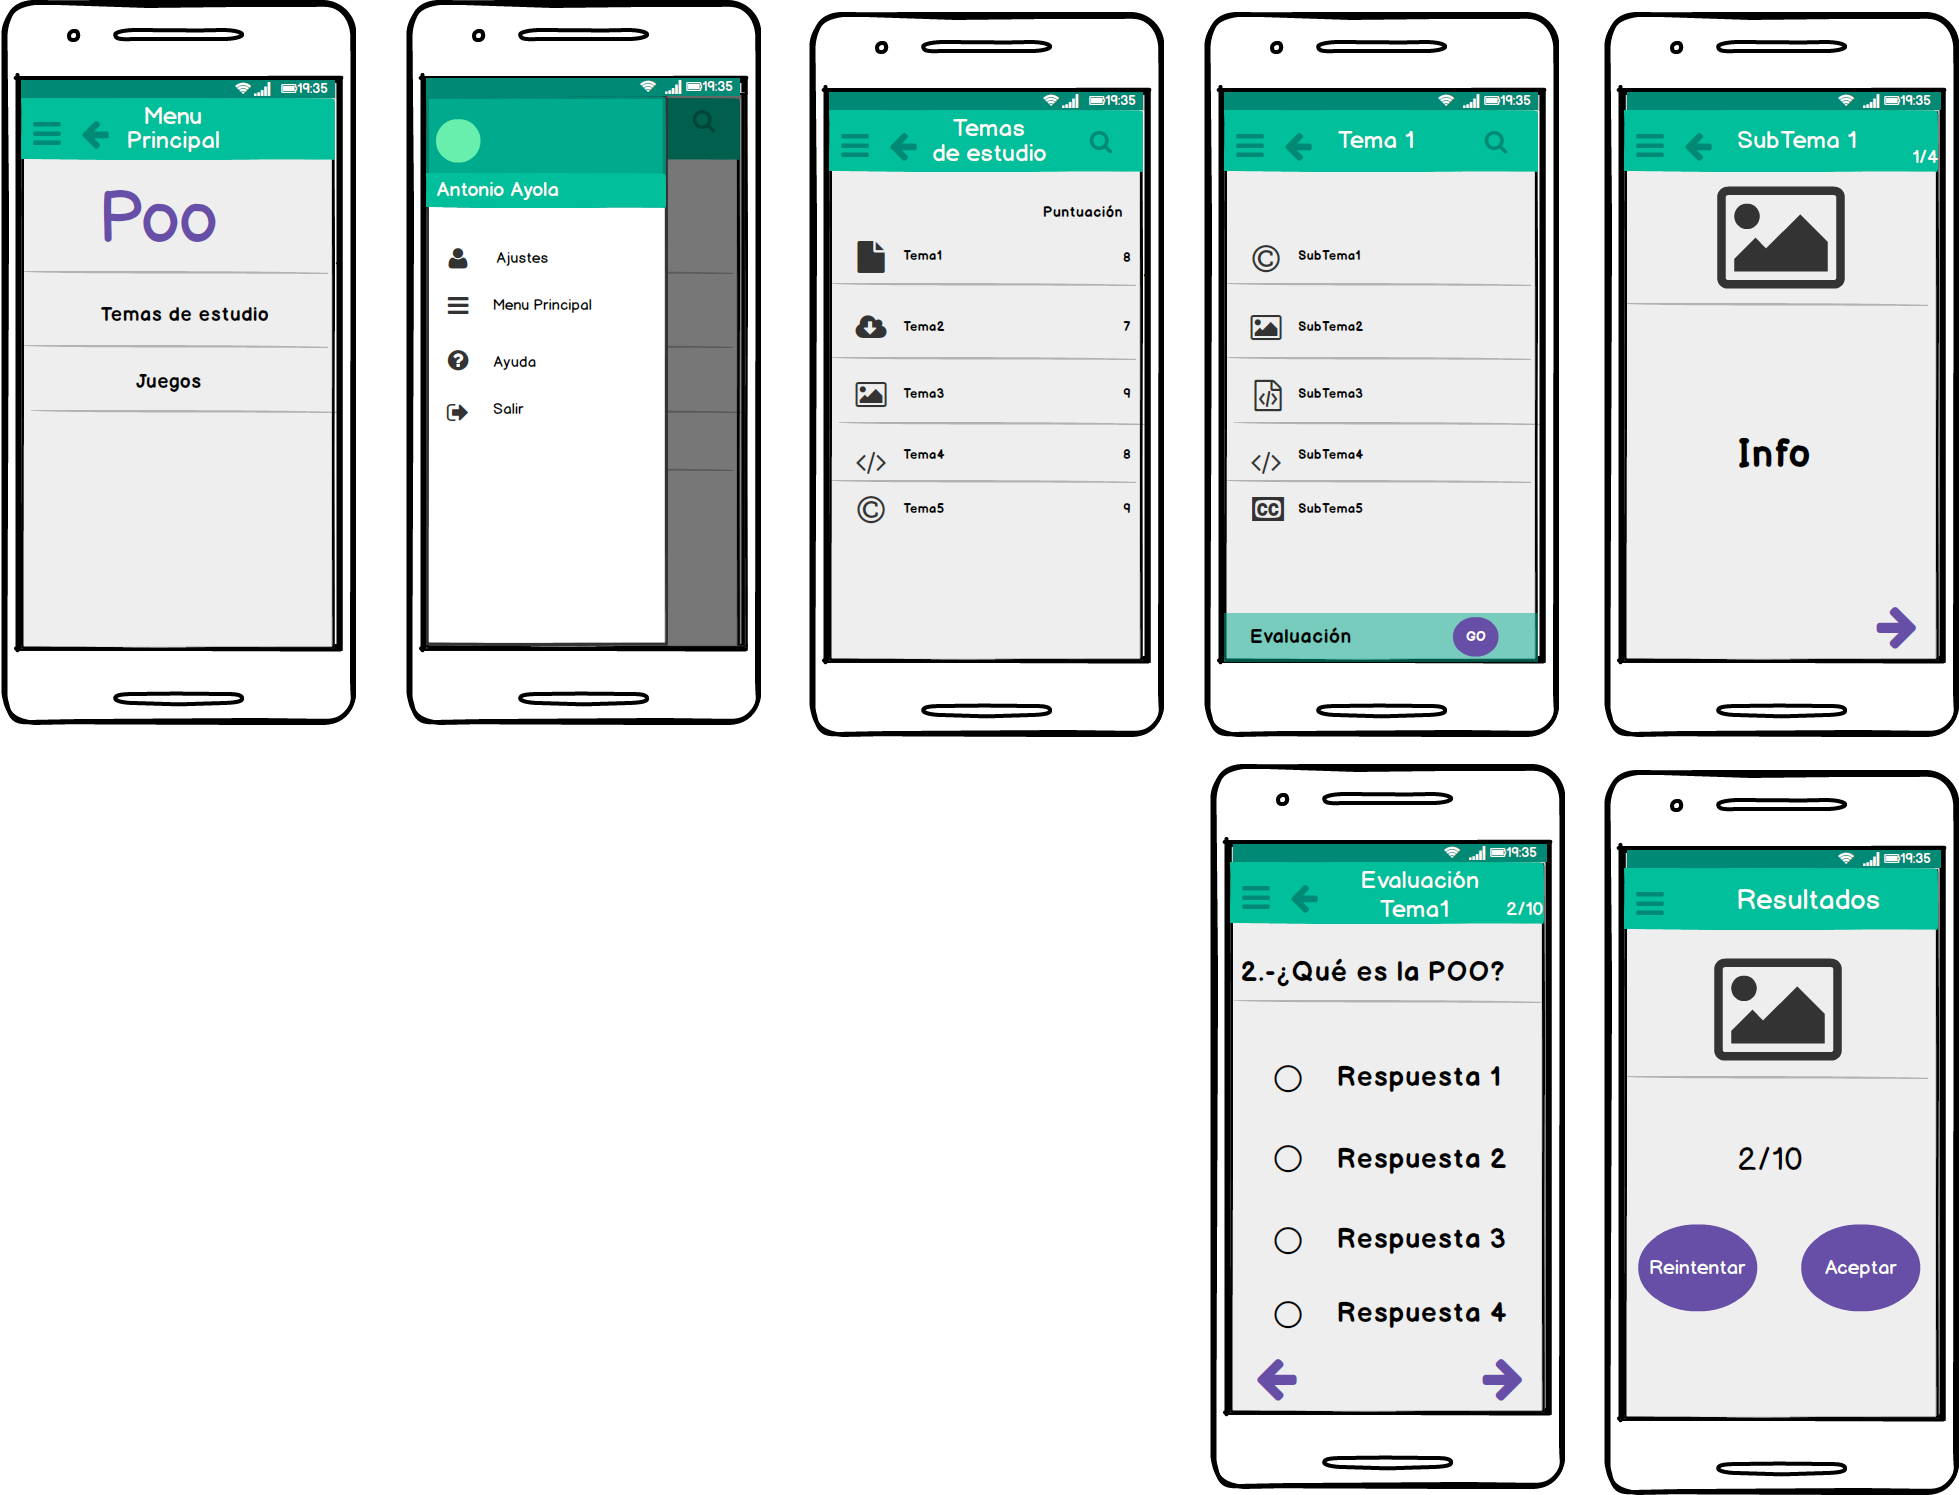
\includegraphics[scale=0.3]{img/m2.png} 
\caption{Pantallas del menú principal, temas, subtemas y evaluación.}
\end{figure}
\end{center}

\begin{center}
\begin{figure}
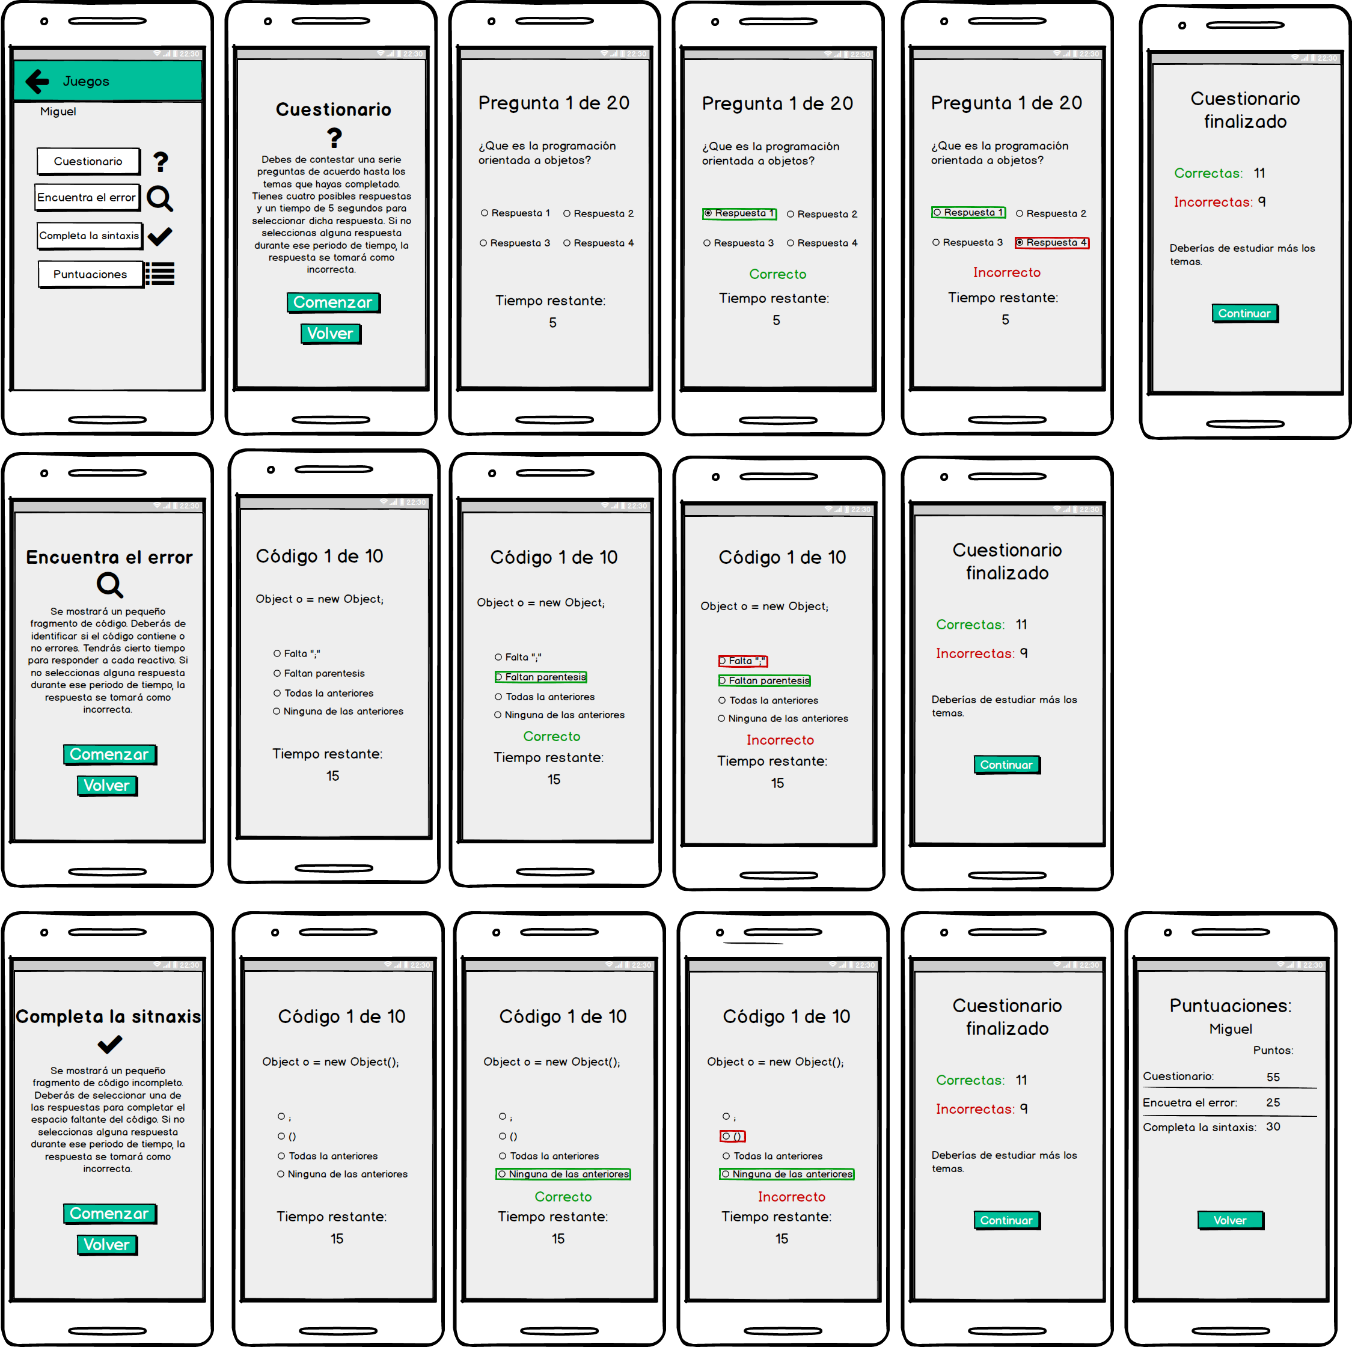
\includegraphics[scale=0.9]{img/m3.png} 
\caption{Pantallas de la sección de juegos}
\end{figure}
\end{center}

\subsection{Diagrama de navegabilidad}

\subsection{Diagrama entidad-relaci'on}

\section{Programaci'on}

\section{Implementaci'on}

\section{Purebas}

\section{Mantenimiento}
